\section*{Chapter 2. Development of an approach to accelerate the fine-tuning through importance analysis}
\addcontentsline{toc}{section}{Chapter 2. Development of an approach to accelerate the fine-tuning through importance analysis}
\setcounter{section}{2} 
\setcounter{subsection}{0}
    The discussed idea of estimating the importance of Transformer blocks formed the basis of the proposed method \ourmethodshort{} (\ourmethodsFull{}). \ourmethodshort{} selectively assigns and re-assigns \lora{} adapters based on Transformer blocks importance during the fine-tuning process with subsequent reduction of the number of Transformer blocks.
    \begin{figure}[H]
        \centering
        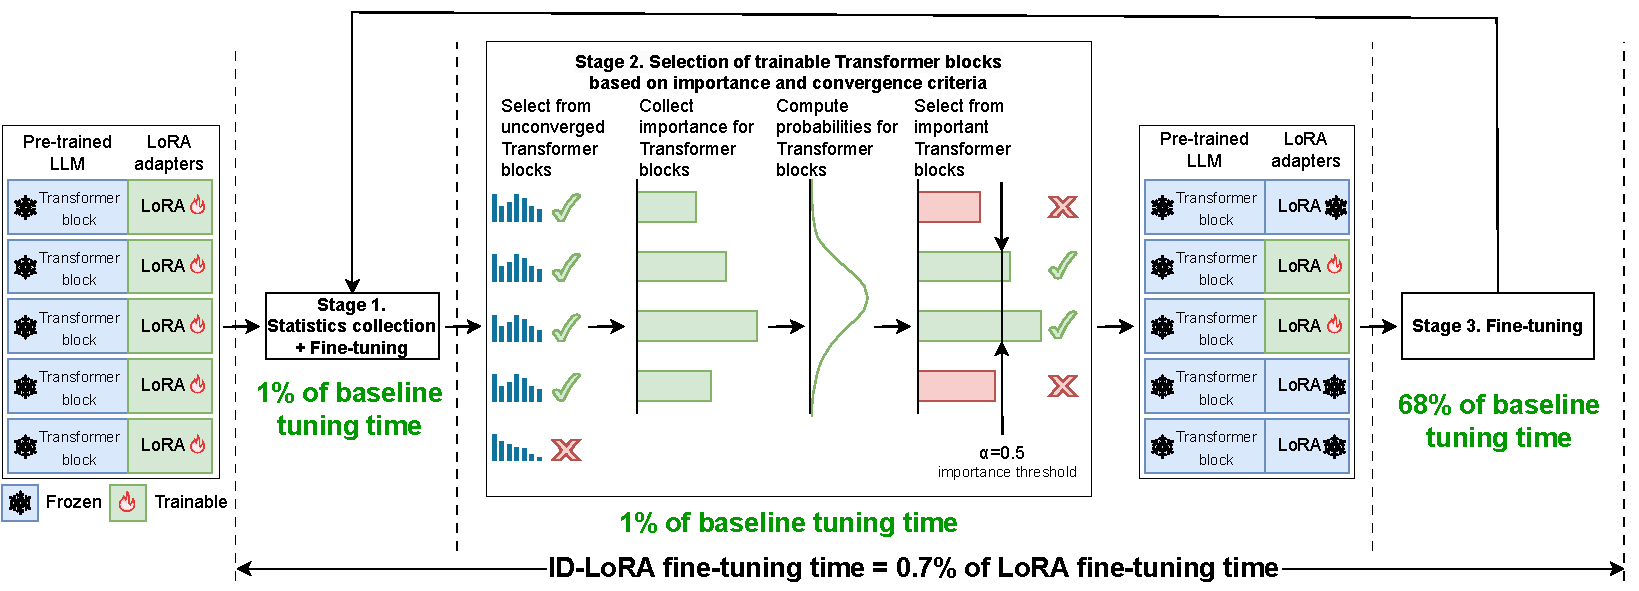
\includegraphics[width=0.99\textwidth]{sections/figures/id_lora.pdf}
        \caption{Key idea of proposed fine-tuning method: \ourmethodsFull{}.}
    \end{figure}
    Let \(h\) denote history defined as the number of steps to collect importance and convergence statistics, \(\alpha\) denote the ratio of Transformer blocks to be selected for fine-tuning.

    Initially, the fine-tuning process is divided into several periods, during which the algorithm switches the trainable Transformer
    blocks. Each \ourmethodshort{} period has 3 stages: statistics collection, selection of trainable Transformer blocks, and fine-tuning of the selected blocks. At the beginning of each stage, layer-wise importance statistic is collected during h steps. Next, algorithm determines unimportant Transformer blocks and removes them from the selection. After that, importance sampling of Transformer blocks is applied, and the ratio of the most important Transformer blocks (\(\alpha\)) is selected for further fine-tuning. At the same time, \lora{} \(A, B\) adapters for not-trainable Transformer blocks are merged up to the end of the fine-tuning. Merging non-updatable adapters allows to further accelerate the fine-tuning process and increase memory reduction. Obviously, with each training period, the number of trainable Transformer blocks diminishes. As a result, fine-tuning stops once there are no more trainable Transformer blocks. As an alternative or a complementary strategy to importance analysis, a convergence analysis was proposed by team to further reduce the number of trainable Transformer blocks. 

    The full \ourmethodshort{} method with importance analysis as my personal contribution and convergence analysis as team proposal is described in Algorithm 1.

    \begin{algorithm}
        \caption{\ourmethodshort{} (\(\alpha, h\))}
        \scriptsize
        \begin{algorithmic}[1]
            \State \(D\): fine-tuning dataset
            \State \(\mathcal{M}_{\Phi}\): pre-trained model
            \State \(\alpha\): trainable blocks selection ratio
            \State \(h\): number of accumulation steps
            \State 
            \State \(C\ \gets \{\} \): converged Transformer blocks 
            \State \(Q \gets \{\mathcal{M}_{\Phi}\} \): trainable Transformer blocks
            \State \(I \gets \{\}\): accumulated importance scores
            \State \(\mathcal{W} \gets \{\} \): accumulated layer weights
            \State \(use\_convergence=True\)
            \For{epoch \(i=1, \dots N\)}
                \For{train step \(i=1, \dots, K\), global batch \(b \in D\)}
                \State \(inp, labels \gets b\): data for forward
                \If{\(i < h\)}
                    \State \textbf{\{Statistics Collection + Fine-tuning Phase\}}
                    \For{layer \(\xi\) in \(\mathcal{M}_{\Phi}\)}
                        \State \(inp, out \gets forward(\xi, inp)\)
                        \State \(I \gets I \cup i(\xi, inp, out)\): calculate layer importance
                        \If{\(use\_convergence\)}
                            \State \(\mathcal{W} \gets \mathcal{W} \cup w_{\xi}\)
                        \EndIf
                        \State \(grads \gets backward(loss(out, labels))\)
                        \State \(apply\_gradients(grads)\)
                    \EndFor
                \ElsIf{\(i=h\)}
                    \State \textbf{\{Selection Phase\}}
                    \For{\(\mathcal{T}\) in \(Q\)}
                        \State \(I_\mathcal{T} \gets I(\{w_j: w_j \in \mathcal{T}\})\): aggregate importance of Transformer blocks (\ref{eq:aggregation})
                        \If{\(use\_convergence\)}
                            \State \(C_{\mathcal{T}} \gets c(\{w_i: w_i \in \mathcal{T}\})\): calculate layer convergence
                        \EndIf
                    \EndFor
                    \State \(T \gets \{\mathcal{T}_i \in Q: C_{\mathcal{T} \ge \varepsilon}\}\)
                    \State \(P \gets softmax(\{I_{\mathcal{T}}: t_{i} \in T\})\): select with (\ref{eq:probability})
                    \State \(T \gets \alpha * top\_p(Q, P)\): (\ref{eq:top-p-sampling})
                    \State \(Unfreeze(R)\)
                    \State \(Freeze(Q \setminus R)\)
                    \State \(Q \gets R\)
                \Else
                    \State \textbf{\{Fine-tuning Phase\}}
                    \State \(inp, out \gets forward(inp)\)
                    \State \(grads \gets backward(loss(out, labels))\)
                    \State \(apply\_gradients(grads)\)
                \EndIf
                \EndFor
            \EndFor
        \end{algorithmic}
    \end{algorithm}
    \subsection{Importance-based Transformer blocks selection}
        \paragraph{Statistics collection phase} The first step of \ourmethodshort{} is dedicated to statistics collection over several iterations of fine-tuning. During \(h\) steps, importance scores are accumulated for each layer of the model. As an importance estimation method several metrics have been considered, including Magnitude rule, Wanda rule, and Cosine Similarity rule. Notably, Magnitude \cite{han2016deepcompressioncompressingdeep} and Wanda \cite{wanda} importance rules are adapted to Transformer block importance estimation as described in Definition \ref{def:transformer-block-importance}.
        \begin{definition}\label{def:transformer-block-importance}
            Let \(T\) denote Transformer blocks, \(i_{\xi}\) denote importance score for \(\xi\) layer inside it, then importance of Transformer block is defined as:
            \begin{equation}\label{eq:aggregation}
                I(T) = \frac{\sum_{\xi \in T} i_{\xi}}{|T|}
            \end{equation}
        \end{definition}
        \paragraph{Selection phase} Upon reaching the \(h\) number of steps, the importance scores of each Transformer block are averaged. After that, the second step of \ourmethodshort{} begins, aimed at selecting important Transformer blocks. Based on the importance scores, selection probability for each Transformer block is computed (\ref{eq:probability}). Next, the Top-P sampling (\ref{eq:top-p-sampling}) is applied, which samples Transformer blocks with the highest probabili-ty scores until the sum of the scores reaches the specified threshold value. Then, the sampling probability for each Transformer block is recalculated (\ref{eq:probability}). Finally, \(\alpha\) of the most important Transformer blocks are selected for further fine-tuning. 
        \begin{equation}\label{eq:probability}
            P(T) = \frac{e^{I(T)}}{\sum_{k=1}^{\mathcal{M}_\Phi}e^{I(k)}},
        \end{equation}
        where \(I\) denotes Transformer block importance score.
        \begin{equation}\label{eq:top-p-sampling}
            Top_P = \{T_k \in \mathcal{M}_\Phi : \sum_{k=1}^{\mathcal{M}_\Phi}P(T_k)\le p\},
        \end{equation}
        where \(p\) denotes the threshold.
    \subsection{Convergence-based Transformer blocks selection}
    Besides the importance analysis, another solution proposed by the team is an optional convergence analysis, which identifies fully trained Transformer blocks that could be frozen, thereby further reducing the number of trainable Transformer blocks. Once per \(h\) steps, additional statistics for convergence analysis are accumulated.
    \begin{definition}\label{def:convergence-rule}
        Let \(\varepsilon\) denote convergence threshold, \(\hat{c}\) denote convergence metric. Then convergence rule for a layer is defined as:
        \begin{equation*}
            c(W_\xi) = 
            \begin{cases}
                1, & \hat{c}(W_\xi) < \varepsilon \\
                0, & \text{otherwise}
            \end{cases}
        \end{equation*}
    \end{definition}
    \begin{definition}\label{def:convergence-inequality}
        Transformer block T is converged if the following inequality with \\ convergence threshold \(\delta\) is satisfied: 
        \begin{equation}
            C(T) = \frac{\sum_{\xi \in T}c(W_{\xi})}{|T|} > \delta
        \end{equation}
    \end{definition}
    When statistic has been collected, the converged Transformer blocks are identified with with the help of convergence rule (\ref{def:convergence-rule}) and corresponding metrics (\ref{def:convergence-inequality}). After that, converged Transformer blocks are frozen up to the end of training, which leads to further reduction of the number of trainable parameters and an earlier stop of the fine-tuning process.
    \subsection{Key differences from existing approaches}
        \begin{itemize}
            \item Current approaches utilizes importance-based pruning of Transformer blocks on inference, introducing considerable quality degradation. In contrast, \ourmethodshort{} integrates the pruning process into the parameter-efficient fine-tuning with \lora{}, thereby preventing performance degradation.
            \item Prior methods incur extra computational costs by requiring inference on calibration data for importance estimation. Conversely, \ourmethodshort{} identifies essential Transformer blocks during the fine-tuning process without additional overhead and calibration data. 
            \item Current state-of-the-art approaches manually attach the \lora{} adapters to all Transformer blocks before the fine-tuning process. On the contrary, \ourmethodshort{} offers an innovative approach that enables automatic assignment of \lora{} \(A, B\) adapters only to important Transformer blocks. 
            \item \ourmethodshort{} applies the idea of additional convergence analysis to further reduce the number of trainable Transformer blocks.
        \end{itemize}
